\documentclass[11pt]{article}
\usepackage[a4paper]{geometry}
\usepackage{mathtools,amssymb,amsthm}
\usepackage{polyglossia}
\usepackage{fontspec}
\usepackage{unicode-math}
\usepackage{titling}
\usepackage{textcomp}
\usepackage{tikz}
\usepackage[shortlabels]{enumitem}

\setdefaultlanguage{french}
\frenchspacing
\setmathfont{Latin Modern Math}
\setmathfont[range={\mathbb,\mathcal,\mathsf}]{xits-math.otf}

\let\oldepsilon\epsilon
\renewcommand\epsilon\varepsilon
\renewcommand\phi\varphi
\newcommand{\N}{\mathbb N}
\newcommand{\Z}{\mathbb Z}
\newcommand{\R}{\mathbb R}
\newcommand{\Q}{\mathbb Q}
\newcommand{\CC}{\mathbb C}
\newcommand{\K}{\mathbb K}
\DeclarePairedDelimiter{\zint}{[\![}{]\!]}

%% Theorem environments
\theoremstyle{definition}
\newtheorem{defn}{Définition}[section]
\newtheorem{prop}[defn]{Proposition}
\newtheorem{axio}[defn]{Axiome}
\newtheorem{exe}{Exemple}
\newtheorem{exo}{Exercice}

\theoremstyle{remark}
\newtheorem{rem}{Remarque}


\begin{document}

\begin{center}
	\hrulefill\\
    \vspace{6mm}
	\textsc{\LARGE Dénombrement}\\
    \vspace{3mm}
    \hrulefill
\end{center}
\vspace{1cm}

\begin{flushright}
<< \textit{...combinatorics, a sort of glorified dice-throwing.} >> \hfill— Robert \textsc{Kanigel}
\end{flushright}

\begin{flushright}
<< \textit{Tout ce dénombrement, madame, est inutile\\
Cent Hectors pourraient-ils me payer un Achille ?} >> \hfill — Pradon, Troade
\end{flushright}


\tableofcontents

\section{Introduction}

\textit{Dénombrer}, c'est compter le nombre d'éléments qu'il y a dans un ensemble, le plus souvent défini par une propriété qu'il vérifie (par exemple, ses éléments pourraient être les parties de $\zint{1,12}$  qui ont $5$...)

Savoir dénombrer permet notamment de faire des calculs de probabilité plus compliquées à la main, et a des applications en physique ou encore en informatique.

Pour démarrer, deux exemples introductifs:

\paragraph{Problème 1} On considère une étagère sur laquelle se situent 4 livres différents.

\begin{figure}[h]
\centering
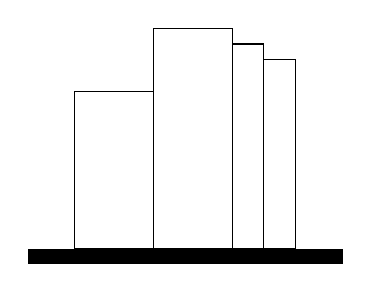
\begin{tikzpicture}
\draw (-1.4,0) rectangle (-0.4,2);
\draw (-0.4,0) rectangle (0.6,2.8);
\draw (0.6,0) rectangle (1.,2.6);
\draw (1.,0) rectangle (1.4,2.4);

\fill (-2,-0.2) rectangle (2,0);
\end{tikzpicture}
\end{figure}

De combien de façons peut-on ranger ces livres ?



\paragraph{Problème 2} On considère maintenant un sac de 10 billes différentes. De combien de façons peut-on constituer un paquet de 4 billes parmi les 10 ?

\section{Applications}

\subsection{Produit cartésien}

\begin{defn}[Produit cartésien]
Soient $E$ et $F$ deux ensembles. On appelle \textit{produit cartésien de $E$ et de $F$}, et on note $E\times F$ (lu << $E$ croix $F$ >>) l'ensemble des couples $(x,y)$ où $x\in E$ et $y\in F$.
\end{defn}

\begin{rem}
En général, $E\times F\neq F\times E$ !
\end{rem}

\begin{exe}\leavevmode
\begin{itemize}

\item $(0,\pi)\in\R\times\R^*$ mais $(0,\pi)\not\in \R^*\times\R$.
\end{itemize}
\end{exe}

\end{document}